\documentclass[a4paper, french]{article}
\usepackage[utf8]{inputenc}
\usepackage{geometry}
\geometry{margin=1.5cm}
\usepackage{ProfLycee}

\begin{document}

\part*{Commandes basiques de \texttt{ProfLycee}}

\section{Outils splinetikz \& tangentetikz}

\begin{center}
	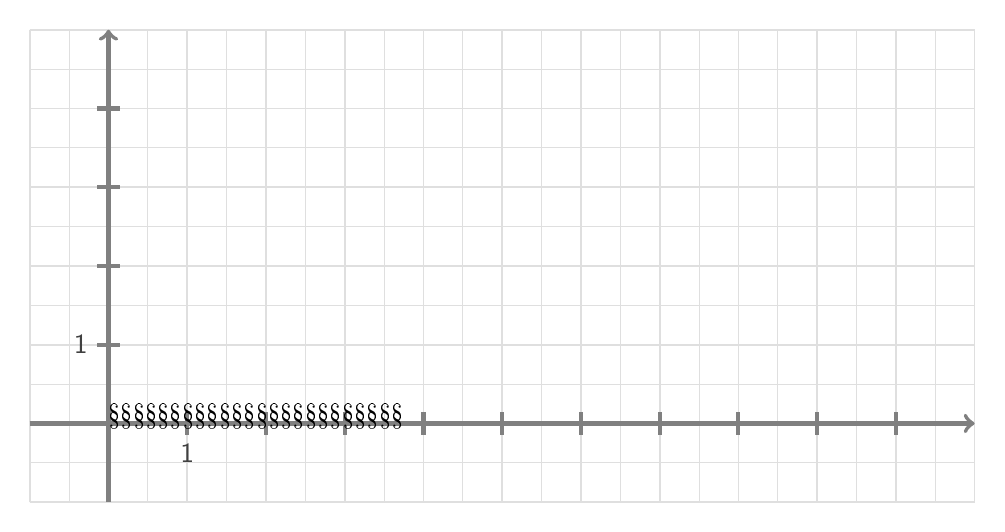
\begin{tikzpicture}
		\draw[xstep=0.5,ystep=0.5,line width=0.3pt,lightgray!50] (-1,-1) grid (11,5);
		\draw[xstep=1,ystep=1,line width=0.6pt,lightgray!50] (-1,-1) grid (11,5) ;
		\draw[line width=1.5pt,->,gray] (-1,0)--(11,0) ;
		\draw[line width=1.5pt,->,gray] (0,-1)--(0,5) ;
		\foreach \x in {0,1,...,10} {\draw[gray,line width=1.5pt] (\x,4pt) -- (\x,-4pt) ;}
		\foreach \y in {0,1,...,4} {\draw[gray,line width=1.5pt] (4pt,\y) -- (-4pt,\y) ;}
		\draw[darkgray] (1,-4pt) node[below,font=\sffamily] {1} ;
		\draw[darkgray] (-4pt,1) node[left,font=\sffamily] {1} ;
		%splines
		\def\LISTE{0/1/0§4/3.667/-0.333§7.5/1.75/0§9/2/-0.333§10/0/-10}
		\splinetikz[liste=\LISTE,affpoints=true,coeffs=3,couleur=red]
		%tangentes
		\tangentetikz[liste=\LISTE,xl=0,xr=1,couleur=ForestGreen,style=dashed]
		\tangentetikz[liste=\LISTE,xl=1,xr=1,couleur=ForestGreen,style=dashed,point=2]
		\tangentetikz[liste=\LISTE,xl=1,xr=1,couleur=ForestGreen,style=dashed,point=3]
		\tangentetikz[liste=\LISTE,xl=1,xr=1,couleur=ForestGreen,style=dashed,point=4]
		\tangentetikz[liste=\LISTE,xl=0.5,xr=0,couleur=ForestGreen,style=dashed,point=5]
	\end{tikzpicture}
\end{center}

\begin{center}
	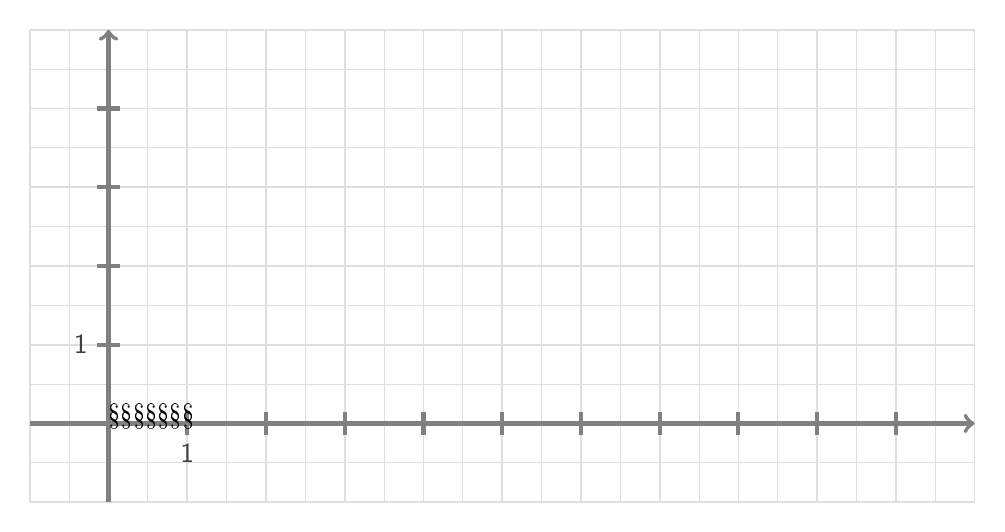
\begin{tikzpicture}
		\draw[xstep=0.5,ystep=0.5,line width=0.3pt,lightgray!50] (-1,-1) grid (11,5);
		\draw[xstep=1,ystep=1,line width=0.6pt,lightgray!50] (-1,-1) grid (11,5) ;
		\draw[line width=1.5pt,->,gray] (-1,0)--(11,0) ;
		\draw[line width=1.5pt,->,gray] (0,-1)--(0,5) ;
		\foreach \x in {0,1,...,10} {\draw[gray,line width=1.5pt] (\x,4pt) -- (\x,-4pt) ;}
		\foreach \y in {0,1,...,4} {\draw[gray,line width=1.5pt] (4pt,\y) -- (-4pt,\y) ;}
		\draw[darkgray] (1,-4pt) node[below,font=\sffamily] {1} ;
		\draw[darkgray] (-4pt,1) node[left,font=\sffamily] {1} ;
		%splines
		\def\LISTE{0/1/0§4/3.667/-0.333§7.5/1.75/0§9/2/-0.333§10/0/-10}
		\splinetikz[liste=\LISTE,affpoints=true,coeffs=3§3§3§2/1,couleur=blue,affpoints=false]
	\end{tikzpicture}
\end{center}

\section{Outils paramCF et ligneCF}

\begin{center}
	\begin{tikzpicture}[x=1cm,y=1cm,line width=1pt]
		\paramCF[titre=true]
		\ligneCF{\textsf{(x+1)\chap2}}{$\mathsf{x^2+2x+1}$}
		\ligneCF{\texttt{(x+1)\chap2}}{$\mathtt{x^2+2x+1}$}
		\ligneCF{\textsf{Dérivée[(x+5)*exp(-0.1*x)]}}{$\mathsf{\rightarrow (0.5-0.1*x)*exp(-0.1*x)}$}
	\end{tikzpicture}
\end{center}

\begin{center}
	\begin{tikzpicture}[x=1cm,y=1cm,line width=1pt]
		\paramCF[titre=false,esplg=0pt,menu=false,couleurcmd=magenta,couleurres=brown,posres=gauche]
		\ligneCF{\textsf{(x+1)\chap2}}{$\mathsf{x^2+2x+1}$}
		\ligneCF{\texttt{(x+1)\chap2}}{$\mathtt{x^2+2x+1}$}
		\ligneCF{\textsf{Dérivée[(x+5)*exp(-0.1*x)]}}{$\mathsf{\rightarrow (0.5-0.1*x)*exp(-0.1*x)}$}
	\end{tikzpicture}
\end{center}

\end{document}